\subsection{\textcolor{blue}{CU 4.1 Agendar Dias}}

\subsubsection{\textcolor{blue}{Resumen}}
Se brinda al usuario turista la posibilidad de crear un nuevo dia para alojar un itinerario mediante el uso de un calendarios.
\subsubsection{\textcolor{blue}{Descripción}}
\begin{tabularx}{16cm}{||l|X||}
	\hline
	\multicolumn{2}{||c||}{Caso de Uso: Agregar Lugares} \\
	\hline
	\multicolumn{2}{||c||}{\textbf{Resumen de atributos}} \\
	\hline
	{Autor:} & Dominguez Olvera Leonardo Daniel \\
    \hline
	{Actor:} & Usuario turista\\
	\hline
	{Próposito:} & Permitir al usuario agendar una fecha para la creación de un nuevo itinerario..\\
	\hline
	{Entradas:}&Se recibe mediante un click agregar dias para crear un itinerario.\\
  &Se recibe mediante un click el dia seleccionado.\\
  & Se recibe mediante un click eliminar uno o todos los dia \\
	\hline
	{Salidas:} &Se mostrara en la pantalla \textcolor{blue}{IU26 Pantalla Dias Itinerario} el mensaje \textcolor{blue}{MSG6 dia ha sido agendado} al agendar un dia.  \\
  & Se mostrara en la pantalla \textcolor{blue}{IU26 Pantalla Dias Itinerario}\\
  &el dia agendado, mostrando su dia.\\
	\hline
	{Precondiciones:} & Debe estar sin agendar la fecha a agendar.\\
	\hline
	{Postcondiciones:}  & Se agenda una fecha para un itinerario\\
	\hline
	{Errores:} & El mes seleccionado no tenga ningun dia disponible se mostrara el mensaje \textcolor{blue}{MSG1 sin fechas disponibles.} \\
 & El dia seleccionado no esta disponible se mostrara el mensaje \textcolor{blue}{MSG Dia no disponible.} \\
  
	\hline
	{Tipo:} & -\\
	\hline
	{Fuente:} & Reunion interna \\
	\hline
	{Observaciones:} & {-} \\
	\hline
\end{tabularx}

\pagebreak
\subsubsection{\textcolor{blue}{Trayectorias del caso de uso}}

\textbf{Trayectoria principal}
\begin{enumerate}

\item 
\includegraphics[width=0.0150\textwidth]{Figuras/persona.png} solicita agregar un itinerario oprimiendo el botón de \textbf{\fbox{+}} de la pantalla \textcolor{blue}{IU26 Pantalla Dias Itinerario}.

\item 
\includegraphics[width=0.0500\textwidth]{Figuras/sistema.png} solicita seleccionar en un calendario el año mostrando la pantalla \textcolor{blue}{IU30 Pantalla Ano Calendario}

\item 
\includegraphics[width=0.0150\textwidth]{Figuras/persona.png} solicita un año oprimiendo el boton \fbox{año} del año correspondiente \textcolor{blue}{[Trayectoria A].}

\item 
\includegraphics[width=0.0500\textwidth]{Figuras/sistema.png} solicita seleccionar en un calendario el mes mostrando la pantalla \textcolor{blue}{IU29 Pantalla Mes Calendario}

\item 
\includegraphics[width=0.0150\textwidth]{Figuras/persona.png} solicita un mes oprimiendo el boton \fbox{mes} del mes correspondiente \textcolor{blue}{[Trayectoria B].}

\item 
\includegraphics[width=0.0500\textwidth]{Figuras/sistema.png} seleccionar en un calendario el mes mostrando la pantalla \textcolor{blue}{IU27 Pantalla Dia calendario}

\item 
\includegraphics[width=0.0150\textwidth]{Figuras/persona.png} un dia oprimiendo la casilla \fbox{dia} del dia correspondiente del calendario.

\item 
\includegraphics[width=0.0500\textwidth]{Figuras/sistema.png} verifica que no se hubiera agendado ese dia previamente de acuerdo a la regla de negocio, \textcolor{blue}{[Trayectoria C].}

\item 
\includegraphics[width=0.0500\textwidth]{Figuras/sistema.png} muestra la pantalla \textcolor{blue}{IU26 Pantalla Dias Itinerario} indicando que el dia fue validado .

\item 
\includegraphics[width=0.0500\textwidth]{Figuras/sistema.png} muestra los mensaje \textcolor{blue}{MSG itinerario vacio y MSG Agregar a intinerario}.

\end{enumerate}
----fin del caso de uso. \\

\subsection{\textbf{Trayectoria A}}

\textbf{Condición:} El usuario turista desea cancelar agendar un calendario \par

     \textbf{A-1} 
\includegraphics[width=0.0150\textwidth]{Figuras/persona.png} oprime el boton \fbox{cancelar}. \\
    \textbf{A-2}
\includegraphics[width=0.0500\textwidth]{Figuras/sistema.png} muestra la pantalla \textcolor{blue}{IU26 Pantalla Dias Itinerario}. \\
   \textbf{A-3} Termina el caso de uso. \\
   ---- Fin de la trayectoria\par


\subsection{\textbf{Trayectoria B}}
\textbf{Condición:} El usuario turista intenta seleccionar un mes sin fechas disponibles.\\
\textbf{B-1} 
\includegraphics[width=0.0500\textwidth]{Figuras/sistema.png} la pantalla \textcolor{blue}{IU29 Pantalla Mes Calendario} el mensaje \textcolor{blue}{MSG sin fechas disponibles.} \\
\textbf{B-2} 
\includegraphics[width=0.0500\textwidth]{Figuras/sistema.png} continua en el paso 3 de la trayectoria principal.\\
-- Fin de trayectoria.\par

\subsection{\textbf{Trayectoria C}}
\textbf{Condición:} El usuario turista intenta seleccionar un dia no disponible\\

\textbf{C-1} 
\includegraphics[width=0.0500\textwidth]{Figuras/sistema.png} muestra la pantalla \textcolor{blue}{Pantalla Dia calendario} el mensaje \textcolor{blue}{MSG2 dia no disponible.} \\
\textbf{C-2} 
\includegraphics[width=0.0500\textwidth]{Figuras/sistema.png} continua en el paso 6 de la trayectoria principal\\
-- Fin de trayectoria.\par\\

\textbf{IU26 Pantalla Dias Itinerario}
\textbf{Objetivo}\\
Obtorgar al usuario turista una herramienta para visualizar, añadir y eliminar los diferentes itinerarios que el requiera.\\

\textbf{Diseño}\\
\begin{figure}[h]
    \centering 
    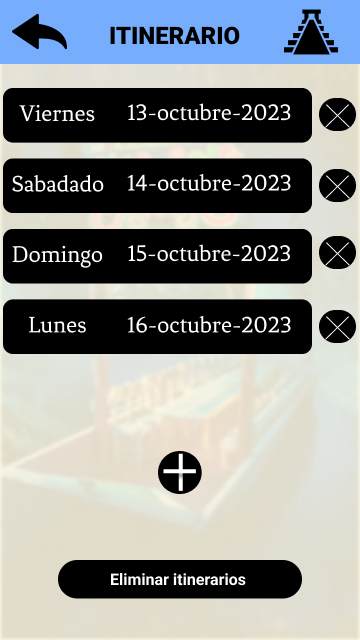
\includegraphics[width=0.5\textwidth]{Pantallas Prototipo3/IU26 Pantalla Dias Itinerario.jpg} 
    \caption{IU26 Pantalla Dias Itinerario} % Agrega el título o descripción de la imagen
    \label{fig:Pantalla de itinerarios} % Etiqueta para referencias cruzadas
\end{figure}

En la figura 1 se muestra la pantalla para agregar los dias a agendar para un nuevo itinerario. Esta pantalla da la opcion de agregar nuevos dias al itinerario, asi como poder visualizar alguno creado y eliminar uno o varios segun se desee.

\textbf{Entradas}\\
\begin{itemize}
    \item Se recibe mediante un click el dia seleccionado.

     \item Se recibe mediante un click agregar dias para crear un itinerario.\\
 \item Se recibe mediante un click eliminar uno o todos los dia \\
\end{itemize}

\textbf{Comandos}\\

\begin{itemize}
    \item \fbox{+}: Agregar dia a iitinerario. Mediante la pantalla \textcolor{blue}{ IU30 Pantalla Ano Calendario.}
    
    \item \fbox{x}: Permite eliminar cada uno de los dias agendados, mediante la pantalla \textcolor{blue}{IU34 Pantalla confirmación eliminar itinerario}
    \item \fbox{Eliminar favoritos}: Permite eliminar los dias agendados, mediante la pantalla \textcolor{blue}{ IU31 Pantalla Eliminar Itinerario}
\end{itemize}

\textbf{Pantallas utilizadas}
\begin{figure}[htb]
    \centering 
        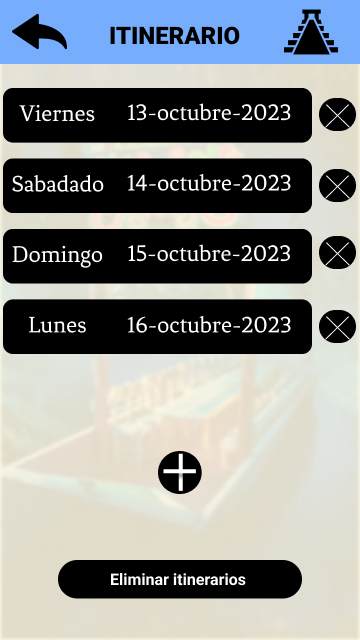
\includegraphics[width=.5\linewidth]{Pantallas Prototipo3/IU26 Pantalla Dias Itinerario.jpg}
        \caption{IU26 Pantalla Dias Itinerario}
\end{figure}
\newpage
\begin{figure}[htb] 
        \centering
        \includegraphics[width=.5\linewidth]{Pantallas Prototipo3/IU30 Pantalla Año Calendario.jpg}
        \caption{IU30 Pantalla Año Calendario}
\end{figure}
\newpage
\begin{figure}[htb]
    \centering 
        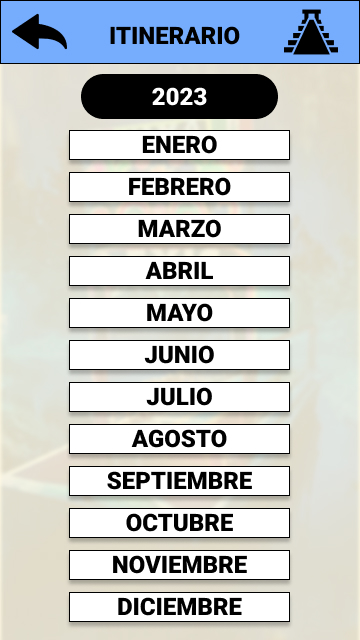
\includegraphics[width=.5\linewidth]{Pantallas Prototipo3/IU29 Pantalla Mes Calendario.jpg}
        \caption{IU29 Pantalla Mes Calendario}
\end{figure}

\newpage
\begin{figure}[htb]
        \centering
        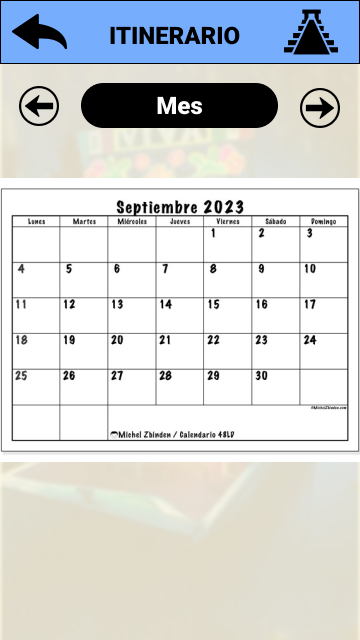
\includegraphics[width=.7\linewidth]{Pantallas Prototipo3/IU28 Pantalla Dia Mes Diferente.jpg}
        \caption{IU28 Pantalla Dia Mes Diferente}
\end{figure}
\newpage
\begin{figure}[htbp]
        \centering
        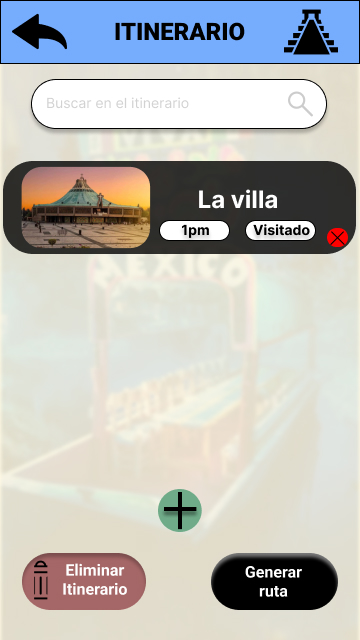
\includegraphics[width= 5cm]{Pantallas Prototipo3/IU33 Pantalla Itinerario Dia.jpg}
        \caption{IU33 Pantalla Itinerario Dia}
        \label{fig:enter-label}
        \vspace{200pt}
\end{figure}